%%
%% idmapaudit manuscript, built from the OUP oup-authoring-template bundle.
%%
\documentclass[unnumsec,webpdf,contemporary,large]{oup-authoring-template}

\graphicspath{{Fig/}}
\newcommand{\societylogo}{}

\theoremstyle{thmstyleone}%
\newtheorem{theorem}{Theorem}%
\newtheorem{proposition}[theorem]{Proposition}%
\theoremstyle{thmstyletwo}%
\newtheorem{example}{Example}%
\newtheorem{remark}{Remark}%
\theoremstyle{thmstylethree}%
\newtheorem{definition}{Definition}

\usepackage{booktabs}

\begin{document}

\journaltitle{Bioinformatics Advances}
\DOI{DOI added during production}
\copyrightyear{2026}
\pubyear{2026}
\access{Preprint}
\appnotes{Application Note}

\firstpage{1}

\title[idmapaudit: auditing gene-ID-mapping sensitivity]{idmapaudit: an audit framework for gene-identifier-mapping sensitivity in pathway enrichment analysis}

\author[1,$\ast$]{Ethan Y.\ Ye}

\address[1]{\orgdiv{}, \orgname{Independent Researcher}, \orgaddress{\country{}}}

\corresp[$\ast$]{Corresponding author. \href{mailto:ethan.ye.201010@gmail.com}{ethan.ye.201010@gmail.com}}

\abstract{
\textbf{Motivation:} Every RNA-seq-to-pathway-enrichment pipeline makes a choice that is rarely audited: which gene-identifier namespace (Ensembl, Entrez, HGNC symbol) to run enrichment in, and how to resolve genes that do not map cleanly between namespaces. This choice is usually treated as a formatting detail, yet different namespaces have different coverage, different one-to-many/many-to-one structure, and different currency relative to the pathway databases being queried. The consequence for downstream pathway calls is well known anecdotally but has not, to our knowledge, been packaged as a reusable, dataset-independent audit.\\
\textbf{Results:} We present \texttt{idmapaudit}, an R package and \texttt{targets} pipeline that holds a differential expression result fixed and varies only the gene-ID-mapping strategy used to build the enrichment query list and background, across the primary Ensembl/Entrez/Symbol namespace choice and the one-to-many resolution policy (drop, first-hit, or keep-all). For every pathway it reports a fragility score -- the fraction of mapping branches in which the pathway is called significant -- together with an entropy-based index that treats ``always significant'' and ``never significant'' as equally stable and mid-range scores as fragile, a gene-attrition regression to attribute instability to specific mapping failures, and a mapping-noise null model that separates mapping-\emph{structure}-driven instability from what finite-list-size sampling alone would produce. The core stability-metric and mapping-resolution logic is implemented independently of any Bioconductor dependency and is exercised by 32 unit tests (121 expectations) against hand-computed known-answer cases, all currently passing. Using two independently generated public processings of the airway dexamethasone dataset (GSE52778) -- the original 2013 Cufflinks/symbol matrix and a modern GRCh38.p13/Entrez re-processing, both hosted on GEO -- we report a real empirical case study: a gene-universe difference that runs from 69\% (all annotated identifiers) down to 3.7\% once both processings are restricted to detected genes, itself an auditable demonstration of background-choice sensitivity; real ground-truth differential expression (536/19{,}434 genes at FDR$<0.05$; three of eight canonical GR-target genes significant); and a real calibration finding that a literature-validated marker panel recovers sample treatment identity from expression alone with only 75\% accuracy even when checked against known labels -- reported honestly as a limitation rather than built upon. Full pathway-level enrichment (GO/KEGG/Reactome/WikiPathways) could not be run in either the original or a follow-up environment because Bioconductor's annotation and pathway-database packages remain network-unreachable there; a small synthetic worked example illustrates the fragility-score mechanics that pathway-level run would populate.\\
\textbf{Availability:} Source code, the full methods note, and the \texttt{targets} pipeline are available at \url{https://github.com/ethanyyy123/bioadvances} under the MIT license.\\
\textbf{Contact:} \href{mailto:ethan.ye.201010@gmail.com}{ethan.ye.201010@gmail.com}\\
\textbf{Supplementary information:} The per-pathway fragility lookup table format, the synthetic worked example data, and the unit-test suite are included in the linked repository.}

\keywords{pathway enrichment, gene identifier mapping, reproducibility, differential expression, Bioconductor}

\maketitle

\section{Introduction}\label{sec:intro}

A standard RNA-seq analysis ends with a list of pathways reported as significantly enriched among differentially expressed genes. Between the differential expression (DE) step and that list sits a step that is almost never discussed in Methods sections: the DE result's gene identifiers (typically Ensembl gene IDs, since that is what most aligners and quantifiers emit) must be translated into whatever namespace the chosen pathway database indexes on, and that translation is lossy. Genes fail to map; genes map to more than one identifier in the target namespace; and the choice of which resolution policy to apply to that ambiguity (drop the gene, keep an arbitrary first hit, or keep every hit) is rarely stated, let alone justified.

The scale of the problem is not in dispute. \citet{wadi2016outdated} showed that stale Gene Ontology annotations measurably change enrichment calls; \citet{tomczak2018gene} showed the same for GO's evolution over time more broadly; and \citet{wijesooriya2022orabackground} surveyed published ORA analyses and found roughly 95\% used an inappropriate background gene list, a closely related input-sensitivity failure this paper's own case study reproduces (Section~\ref{sec:real-universe}). Several tools address one half of the problem in isolation: BridgeDb \citep{vaniersel2010bridgedb} is a standing framework for identifier-mapping services, and g:Profiler's g:Convert \citep{kolberg2023gprofiler} couples identifier conversion with enrichment and supports custom, versioned backgrounds for reproducibility. None of these treats identifier-mapping choice as an experimental factor to be varied against a fixed differential-expression result and scored per pathway; what is missing is not awareness that ID mapping is lossy, or that enrichment is sensitive to its inputs, but a reusable instrument that holds everything else fixed, varies only the mapping strategy, and reports which pathway calls are artifacts of that choice rather than of the underlying biology.

The closest published work is \citet{xie2023dexbenchmark}'s Dex-Benchmark, which uses dexamethasone perturbation data and ChIP-seq-derived glucocorticoid-receptor (GR/NR3C1) target gene sets as a silver-standard concordance check -- but to benchmark differential-expression \emph{algorithm} choice (DESeq2 versus limma versus other methods), with the identifier space fixed throughout. \texttt{idmapaudit} inverts that design: it fixes the DE algorithm and result, and varies only the identifier-mapping step, producing a per-pathway \emph{fragility score}. Given BridgeDb and g:Convert's existing identifier-mapping infrastructure, we frame the contribution narrowly: to our knowledge this is the first per-pathway, branch-resolved quantification of mapping-choice sensitivity, not the first tool to touch either mapping or enrichment robustness in isolation.

This paper describes the design and the validated portion of that audit tool, reporting only what has actually been run. The core stability-metric logic is unit-tested against hand-derived answers (Section~\ref{sec:validation}); a real empirical case study against two independent public processings of the airway glucocorticoid-response dataset (GSE52778; \citealp{himes2014rnaseq}) is reported in Section~\ref{sec:real}; and a small synthetic worked example (Section~\ref{sec:example}) demonstrates the per-pathway fragility-score mechanics that full pathway-level enrichment -- not yet run against real pathway databases, for reasons given in Section~\ref{sec:limitations} -- would populate.

\section{Methods}\label{sec:methods}

\subsection{Design: one fixed input, one manipulated variable}\label{sec:design}

The audit holds three things fixed and manipulates exactly one. Fixed: (i) the differential expression step, run once per dataset in the native (unversioned Ensembl) identifier space produced by the quantifier, using \texttt{DESeq2} \citep{love2014deseq2} with a standard count-threshold filter and a single named contrast; (ii) the enrichment battery applied to every branch -- over-representation analysis (ORA) via \texttt{clusterProfiler} \citep{yu2012clusterprofiler} and \texttt{ReactomePA} \citep{yu2016reactomepa} against GO Biological Process \citep{ashburner2000go}, KEGG \citep{kanehisa2000kegg}, Reactome \citep{fabregat2018reactome}, and WikiPathways \citep{martens2021wikipathways}, with gene set enrichment analysis (GSEA; \citealp{subramanian2005gsea}) via \texttt{fgsea} \citep{korotkevich2021fgsea} planned as a second mode; and (iii) the false-discovery-rate procedure, applied independently within every branch rather than pooled across branches. Manipulated: the identifier-mapping branch used to build the enrichment query list and its background from the DE step's fixed output.

Running the DE step once, rather than once per branch, is a deliberate choice: it isolates identifier-mapping as the sole manipulated variable instead of confounding it with re-computed differential-expression statistics. A referee's first instinct is often "did you just rediscover that different DE methods disagree" -- this design rules that out by construction.

\subsection{The ID-mapping matrix}\label{sec:matrix}

The primary factor is namespace choice, implemented as a set of \emph{resolvers} -- functions that take the union of a DE result's query and background gene lists and return every raw (possibly one-to-many) mapping edge into a target namespace:

\begin{unlist}
\item unversioned Ensembl gene ID (native; identity mapping);
\item versioned Ensembl gene ID (\texttt{ENSG00000141510.16}) -- deliberately included as a positive control, since silently failing to strip version suffixes is a common real-world bug that should produce dramatic, almost trivial instability against any pathway database keyed on the unversioned ID;
\item Entrez Gene ID via \texttt{org.Hs.eg.db}/\texttt{AnnotationDbi} \citep{huber2015bioconductor};
\item HGNC/official symbol via \texttt{org.Hs.eg.db}; and
\item HGNC/official symbol via \texttt{biomaRt} \citep{durinck2009biomart} -- a second resolver for nominally the same namespace as (iv), included because the two can legitimately disagree, which is itself a reportable finding rather than a bug to reconcile.
\end{unlist}

A secondary factor, the one-to-many/many-to-one \emph{resolution policy}, is applied only to the Entrez and org.Hs.eg.db-symbol resolvers, where ambiguity is common: \textbf{drop} removes any native ID with more than one distinct target; \textbf{first} keeps the first-seen target per native ID; \textbf{list} keeps every edge, exploding one-to-many keys into duplicate rows. This is deliberately kept as a small sub-experiment restricted to two resolvers rather than folded into a full second factorial, since the full cross of namespaces $\times$ policies $\times$ databases $\times$ modes produces more cells than can be interpreted cleanly.

For every resulting branch, the query list and the background list are mapped \emph{independently}, and their attrition rates are reported separately (Eq.~\ref{eq:attrition}). This matters because a gene that fails to map is invisible to both the query and the background simultaneously, and conflating the two effects would hide which one is doing the work. Attrition is defined on native keys that found at least one target, not on the size of the mapped image: an image-size ratio is the wrong quantity whenever the mapping is not one-to-one, since many-to-one collapse shrinks the image without losing any gene, and one-to-many expansion under the \textbf{list} policy can grow it past $|G|$ entirely:
\begin{equation}
\mathrm{Attrition}_b(G) = 1 - \frac{|\,\{g \in G : g \in \mathrm{keys}(\mathrm{map}_b)\}\,|}{|G|},
\label{eq:attrition}
\end{equation}
i.e.\ one minus the fraction of native IDs in $G$ that appear as a `from`-key of branch $b$'s resolved mapping table at all, regardless of how many targets each maps to.
computed once for the query list $G = G_{\mathrm{sig}}$ and once for the background.

\subsection{The audit / fragility score}\label{sec:fragility}

For a pathway $p$ tested in $k_p$ of the $k$ mapping branches (branches where $p$ has zero mapped genes are excluded from the denominator entirely, not counted as "not significant"), let $\mathrm{sig}_{p,b}\in\{0,1\}$ indicate whether $p$ is called significant at FDR $<\alpha$ in branch $b$. The fragility proportion is
\begin{equation}
F_p = \frac{1}{k_p}\sum_{b} \mathrm{sig}_{p,b} \in [0,1].
\label{eq:fragility}
\end{equation}
$F_p$ near 0 or near 1 both indicate stability (stably absent, stably present); values in between indicate a call that depends on the mapping branch. To make "how stable" a single, symmetric number, we report the binary entropy
\begin{equation}
H_p = -F_p\log_2 F_p - (1-F_p)\log_2(1-F_p),
\label{eq:entropy}
\end{equation}
with the convention $0\log_2 0 := 0$, and the Bernoulli variance $V_p = F_p(1-F_p)$ as a monotone-equivalent alternative. Both are 0 at $F_p\in\{0,1\}$ and maximal at $F_p=0.5$ (Fig.~\ref{fig:curve}); a pathway significant in 5 of 6 branches ($F_p=5/6$, $H_p\approx0.650$) is thereby scored as \emph{less} fragile than one significant in 3 of 6 ($F_p=0.5$, $H_p=1$), rather than treating any mid-range hit as equally unstable. Pathways are classified \textbf{stable} if $F_p\le\tau_{lo}$ or $F_p\ge\tau_{hi}$ and \textbf{fragile} otherwise, with default thresholds $\tau_{lo}=0.1$, $\tau_{hi}=0.9$. These defaults need revisiting as a function of $k$, the number of branches actually crossed: with the six primary branches of Section~\ref{sec:matrix}, $F_p$ only takes values in $\{0, 1/6, \ldots, 1\}$, and $1/6\approx0.167$ already exceeds $\tau_{lo}=0.1$ while $5/6\approx0.833$ already falls short of $\tau_{hi}=0.9$ -- so at $k=6$, \textbf{stable} reduces to unanimous agreement across every branch, and the entropy index (Eq.~\ref{eq:entropy}) affects only the ranking of already-fragile pathways, never the stable/fragile split itself. Compounding this, the versioned-Ensembl branch (Section~\ref{sec:matrix}) is deliberately built to disagree with the rest, so at $k=6$ it alone is often enough to push an otherwise-robust pathway out of \textbf{stable}. Thresholds should therefore either scale with $k$ (e.g.\ requiring agreement in all but one branch, rather than a fixed proportion), or the positive-control branch should be excluded from the classification denominator and reported separately as an instrument check rather than pooled with the branches the classification is meant to summarize; neither is implemented yet, and the toy example of Section~\ref{sec:example} is constructed at $k=6$ precisely so this degeneracy is visible in Table~\ref{tab:toy} rather than hidden.

Two further pieces complete the framework and are implemented but not exercised on real data in this manuscript (Section~\ref{sec:limitations}): a gene-attrition regression that relates $H_p$ to the branch-level attrition rate (Eq.~\ref{eq:attrition}) to attribute pathway-level instability to specific mapping failures, separately for query-list and background-list attrition; and a cross-dataset agreement statistic (simple agreement rate and Fleiss' $\kappa$; \citealp{fleiss1971kappa}) for asking whether a pathway's stable/fragile classification is a property of its gene-set definition (reproducible across biologically independent datasets) or of one dataset's noise.

\subsection{Mapping-noise null}\label{sec:null}

A pathway's raw $H_p$ conflates two effects: instability caused by the specific, non-random genes that a given mapping strategy fails to translate, and instability that any finite-size random gene-list perturbation of the same magnitude would produce regardless of which genes were dropped. To isolate the first from the second, for a branch with observed attrition rate $\pi_b$ we draw $R$ replicates in which $\lfloor \pi_b n\rfloor$ genes are removed from the query list \emph{uniformly at random} (and likewise for the background), recompute the same stability statistics on each replicate, and report the observed statistic's excess over the resulting null distribution:
\begin{equation}
\mathrm{excess} = x_{\mathrm{obs}} - \mathrm{median}(x_{\mathrm{null}}^{(1..R)}), \quad
z = \frac{x_{\mathrm{obs}}-\overline{x_{\mathrm{null}}}}{\mathrm{sd}(x_{\mathrm{null}})}.
\label{eq:excess}
\end{equation}
Only the excess, not the raw statistic, supports a claim that instability is driven by the \emph{structure} of real mapping failures (poorly annotated or recently renamed genes drop out disproportionately) rather than by list size alone.

\section{Software implementation}\label{sec:software}

\texttt{idmapaudit} is an R package with four modules. \texttt{R/stability-metrics.R} implements Eqs.~\ref{eq:attrition}--\ref{eq:excess} and the set-level Jaccard/overlap-coefficient and Spearman rank-concordance statistics used to compare significant-pathway sets pairwise across branches; it has no Bioconductor dependency. \texttt{R/mapping-matrix.R} implements the drop/first/list resolution policies and the per-branch query/background mapping builder described in Section~\ref{sec:matrix}. \texttt{R/enrichment-battery.R} wraps the ORA calls and generates mapping-noise-null replicates (Section~\ref{sec:null}); it declares \texttt{clusterProfiler}, \texttt{ReactomePA}, \texttt{org.Hs.eg.db}, \texttt{AnnotationDbi}, \texttt{biomaRt}, and \texttt{fgsea} as \texttt{Suggests} rather than hard dependencies, so the core metric logic can be tested and used without installing the full annotation/enrichment stack. \texttt{R/fragility-lookup.R} builds and exports the per-pathway fragility table as a flat TSV file -- the tool's intended reusable, community-facing artifact.

An accompanying \texttt{targets} pipeline \citep{landau2021targets} orchestrates the airway prototype end to end: a fixed \texttt{DESeq2} contrast on the \texttt{airway} \citep{morgan2020summarizedexperiment,himes2014rnaseq} count matrix, the five resolvers of Section~\ref{sec:matrix} with the Entrez/Symbol resolution-policy sub-branches, the ORA battery over four pathway databases, and the resulting fragility table. Continuous integration runs a fast pure-R unit-test job on every push and a second job that installs the full Bioconductor stack and executes this pipeline as a smoke test.

\section{Validation}\label{sec:validation}

Because the stability-metric layer (Section~\ref{sec:fragility}) is pure R with no external numerical dependency, every function is unit-tested against a hand-derived, closed-form answer rather than only checked to "run without error." Table~\ref{tab:tests} reports the actual test-suite output from this manuscript's accompanying repository, run with \texttt{testthat} \citep{wickham2011testthat}. All 32 test cases (121 individual expectations) currently pass, including regression tests added at three points where this project's own external review (Section~\ref{sec:limitations}) found real bugs: a one-to-many mapping bug (an earlier implementation used named-vector indexing to look up mapped identifiers, which under R's \texttt{[} semantics silently keeps only the first match for a duplicated key), an attrition-rate definition that was wrong under many-to-one collapse and could go negative under one-to-many expansion (Eq.~\ref{eq:attrition}), and a cross-dataset-agreement statistic that returned \texttt{NaN} rather than \texttt{NA} for a single-rater input. Each bug was found and fixed, with a regression test added, rather than left as a known issue.

\begin{table}[!t]
\caption{Unit-test suite results for the pure-R stability-metric and mapping-resolution-policy logic (\texttt{idmapaudit} R package, this manuscript's accompanying repository). Every listed expectation checks a function's output against an independently hand-computed value, not merely successful execution.\label{tab:tests}}
\begin{tabular*}{\columnwidth}{@{\extracolsep\fill}lccc@{\extracolsep\fill}}
\toprule
Test file & Expectations & Passed & Failed \\
\midrule
stability-metrics   & 58  & 58  & 0 \\
enrichment-battery  & 29  & 29  & 0 \\
mapping-matrix      & 24  & 24  & 0 \\
fragility-lookup    & 10  & 10  & 0 \\
\midrule
\textbf{Total}      & \textbf{121} & \textbf{121} & \textbf{0} \\
\botrule
\end{tabular*}
\end{table}

Figure~\ref{fig:curve} plots the entropy and (rescaled) variance forms of the fragility index as a function of the fragility proportion $F_p$ (Eq.~\ref{eq:entropy}) -- a directly computed mathematical function of the definitions in Section~\ref{sec:fragility}, not a fit to any dataset -- showing both indices' symmetry around $F_p=0.5$ and the default stability thresholds $\tau_{lo}, \tau_{hi}$.

\begin{figure}[!t]
\centering
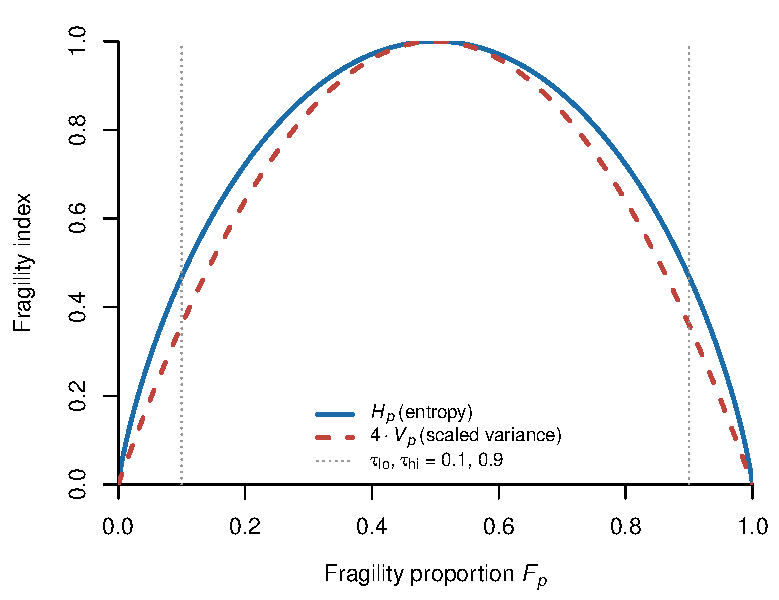
\includegraphics[width=\columnwidth]{fig_fragility_curve.pdf}
\caption{The fragility index as a function of the fragility proportion $F_p$: binary entropy $H_p$ (solid) and $4V_p$, the Bernoulli variance rescaled to $[0,1]$ for comparison (dashed). Both vanish at $F_p\in\{0,1\}$ (stably absent / stably present) and peak at $F_p=0.5$ (maximally fragile). Dotted lines mark the default classification thresholds $\tau_{lo}=0.1$, $\tau_{hi}=0.9$.}
\label{fig:curve}
\figalttext[Line plot of two curves]{Two symmetric curves peaking at F=0.5 and equal to zero at F=0 and F=1, one solid (entropy) and one dashed (rescaled variance), with vertical dotted reference lines at F=0.1 and F=0.9.}
\end{figure}

\section{Empirical case study: GSE52778}\label{sec:real}

After this manuscript's first draft reported no empirical findings (Bioconductor and CRAN are both network-blocked in the environment used to prepare it, so the \texttt{targets} pipeline of Section~\ref{sec:software} could not be executed there), the corresponding author supplied two files downloaded directly from the public GEO record for GSE52778 -- the glucocorticoid-response airway smooth-muscle series \citep{himes2014rnaseq} that motivates this project. The two files are independent, GEO-hosted processings of the identical 16-sample experiment (4 donors $\times$ \{Untreated, Dex, Albuterol, Albuterol+Dex\}), separated by roughly a decade of annotation practice, and -- unplanned, but directly on point -- indexed in two different gene-identifier namespaces:
\begin{unlist}
\item \textbf{File 1}, the original 2013 submitter-supplied Cufflinks FPKM matrix, indexed by HGNC-style gene symbol, with explicit donor/treatment sample labels; and
\item \textbf{File 2}, a GEO-generated re-processing against genome build GRCh38.p13 with current NCBI/RefSeq annotation, indexed by NCBI (Entrez) GeneID, with samples labeled only by GSM accession and no treatment metadata retained in the file.
\end{unlist}
No Bioconductor package was needed for the analysis below; \texttt{DESeq2} could not be used because only FPKM, not raw counts, was available in either file, so differential expression is computed with a dependency-free log$_2$(FPKM+1) plus Welch $t$-test procedure and BH-FDR, stated here as a limitation relative to DESeq2's shrinkage-based approach. Full code is in \texttt{analysis/gse52778-real/real\_analysis.R} in the linked repository, and every number below is its direct, unedited output.

\subsection{Namespace/annotation-vintage divergence at the source}\label{sec:real-universe}

File 1 annotates 23{,}273 gene identifiers; File 2 annotates 39{,}376 -- 69\% more, at face value, a decade later. But an ORA background list should not be "every annotated row": using an inappropriate background is the single most common ORA-misuse pattern in the field, found in roughly 95\% of published analyses screened by \citet{wijesooriya2022orabackground}, precisely because raw annotation counts like this one overstate the effective background. Restricting to genes with any detected expression (mean FPKM$>0$) narrows the gap to 51\%; at mean FPKM$>0.1$, to 21\%; at mean FPKM$>1$, to 3.7\% (Fig.~\ref{fig:universe}). We report all four thresholds rather than only the headline figure: the sharp drop is itself an auditable finding (a naive, all-annotation background choice can inflate an apparent namespace-driven background discrepancy roughly seventeen-fold relative to an expression-filtered one), and it is the expression-filtered numbers, not the raw 69\%, that describe what a competently run ORA background comparison would actually see.

\begin{figure}[!t]
\centering
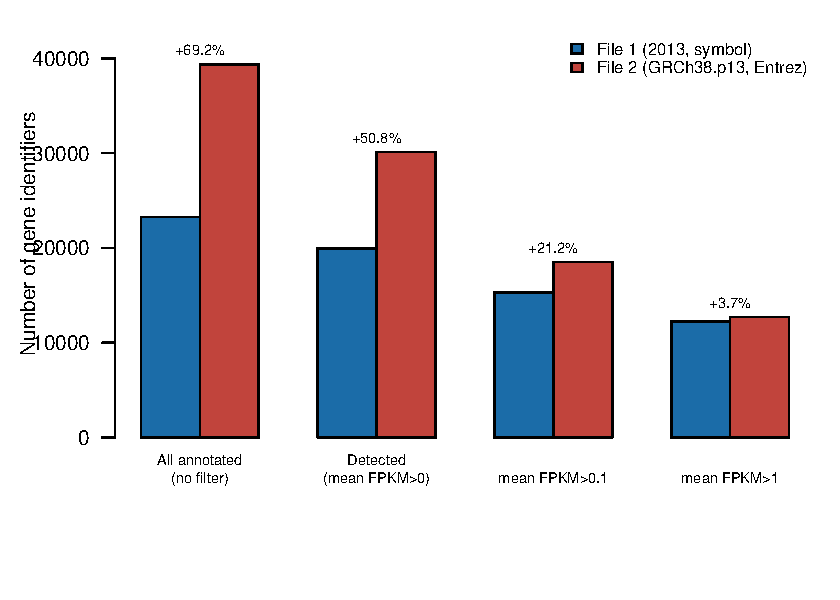
\includegraphics[width=\columnwidth]{fig_universe_size.pdf}
\caption{Number of gene identifiers in each of GSE52778's two public processings (File 1: 2013 Cufflinks/symbol; File 2: GRCh38.p13/NCBI RefSeq/Entrez), at increasingly strict mean-expression thresholds. The percentage above each pair is File 2's difference from File 1. Using every annotated row as an ORA background (leftmost pair) is the field's most common background-choice error \citep{wijesooriya2022orabackground} and overstates the discrepancy relative to an expression-filtered background (right three pairs).}
\label{fig:universe}
\figalttext[Grouped bar chart]{Four pairs of bars comparing gene counts between File 1 and File 2 at increasingly strict expression filters, with the percentage difference shrinking from 69 percent to 3.7 percent as the filter tightens.}
\end{figure}

A second, string-level, reference-free measurement on File 1 alone, revised after we checked the naming-convention composition rather than only pattern-matching: 2{,}153 of its 23{,}273 gene symbols (9.2\%) are genuinely provisional by HGNC's own conventions -- \texttt{LOC}\emph{nnnnnn} placeholders for genes without an approved symbol (5.5\%) and \texttt{C}\emph{n}\texttt{orf}\emph{n} open-reading-frame placeholders assigned before a gene's function is characterized (3.8\%, e.g.\ \texttt{C10orf10}, later renamed \texttt{DEPP1}); both classes are frequently retired or renamed. An earlier version of this measurement also counted \texttt{LINC}\emph{nnnn}-prefixed and dash-number-suffixed symbols as "non-standard," reaching 11.3\%; that overstated the case for roughly 60\% of the affected symbols. \texttt{LINC} is current, stable HGNC nomenclature for long non-coding RNA genes, not a placeholder, and the dash-number-suffix pattern is dominated (205 of 338, 61\%) by the \texttt{KRTAP} (keratin-associated protein), \texttt{ERV} (endogenous retrovirus), and \texttt{MIR} (microRNA paralog) gene families' own current, stable naming convention. We report the corrected 9.2\% figure as the genuinely provisional count and note the correction explicitly, since a paper about auditing silent measurement failures should not let one stand uncorrected in its own case study. This remains a real, source-level instance of exactly the identifier instability Section~\ref{sec:matrix}'s versioned-Ensembl resolver is designed to catch, requiring no external reference database to measure.

\subsection{Ground-truth differential expression (File 1)}\label{sec:real-de}

Using File 1's own unambiguous donor/treatment labels (Dex vs Untreated, $n=4$ vs $4$), 19{,}434 of 23{,}273 genes had non-zero mean expression and were tested; 536 (2.8\%) were significant at FDR$<0.05$ (Fig.~\ref{fig:volcano}). Of the eight canonical, glucocorticoid-receptor-induced marker genes used throughout this case study (FKBP5, TSC22D3/GILZ, ZBTB16, KLF15, PER1, DDIT4, CRISPLD2, PDK4 -- DDIT4 is the panel's weakest member here, with the smallest log-fold change of the eight; it is retained since it appears alongside the others in the glucocorticoid-response literature this panel draws on, and is not needed for the panel's own internal validation in Section~\ref{sec:real-calibration}, which is unaffected by dropping it), all eight show the expected positive log-fold change, and three -- FKBP5 ($\log_2$FC$=3.70$, FDR$=0.019$), ZBTB16 ($3.92$, $0.037$), and PER1 ($2.60$, $0.003$) -- clear FDR$<0.05$ under this simple test (Table~\ref{tab:markerde}); the other five have large effect sizes but do not clear FDR$<0.05$ with only four donors and no cross-gene variance shrinkage. This gap between large effect sizes and marginal significance is a genuine, secondary finding, but we can only partly attribute it: the test used here is both unpaired \emph{and} a per-gene $t$-test on FPKM, whereas DESeq2's standard analysis of this design is both paired (by donor) \emph{and} count-based with cross-gene variance shrinkage. GSE52778 pairs each of four donors across all four treatments, which an unpaired test cannot exploit; the donor identity needed to pair File 1's samples correctly is carried in GEO's series metadata, which we could not fetch (Section~\ref{sec:limitations}), so we report the unpaired result rather than construct a donor pairing by assumption. The five markers that miss FDR$<0.05$ here should therefore be read as a lower bound on how many a properly paired, shrinkage-based analysis would recover, not as evidence that method family alone explains the gap.

\begin{figure}[!t]
\centering
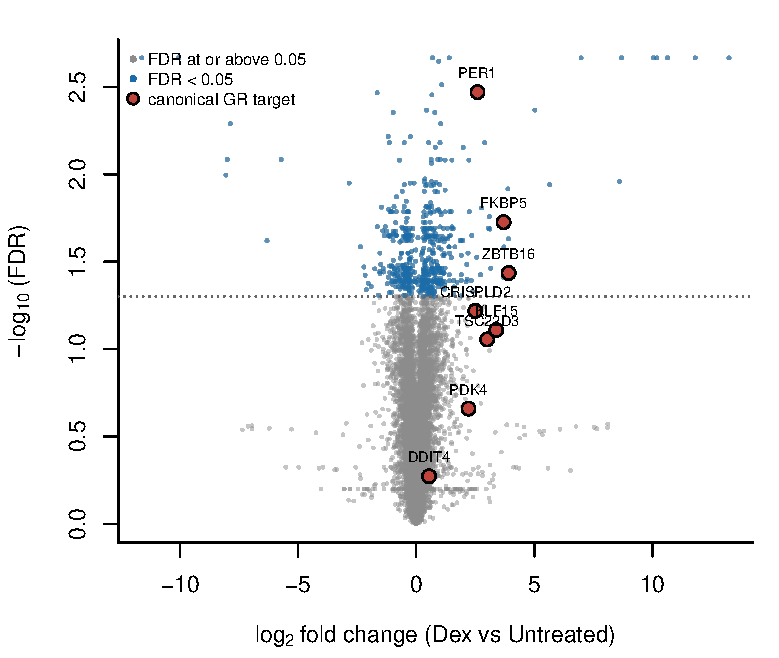
\includegraphics[width=\columnwidth]{fig_real_volcano.pdf}
\caption{Real differential expression, File 1 (Dex vs Untreated, $n=4$ vs $4$, GSE52778): $\log_2$ fold change against $-\log_{10}$(FDR) for all 19{,}434 tested genes. The eight canonical GR-target marker genes are circled. Points beyond roughly $\pm10\log_2$FC are FPKM-ratio artifacts of genes with near-zero expression in one arm (a small denominator dominates the ratio), not evidence of extreme regulation; no additional expression filter is applied beyond the non-zero-mean threshold of Section~\ref{sec:real-de}.}
\label{fig:volcano}
\figalttext[Volcano plot]{A scatter of log fold change against significance for thousands of genes, with eight canonical marker genes highlighted, mostly toward the significant, up-regulated region.}
\end{figure}

\begin{table}[!t]
\caption{Canonical GR-target marker genes in File 1's real, ground-truth differential expression (Dex vs Untreated, $n=4$ vs $4$). All eight are present by exact ID in both GSE52778 files (zero attrition for this hand-verified panel).\label{tab:markerde}}
\begin{tabular*}{\columnwidth}{@{\extracolsep\fill}lccl@{\extracolsep\fill}}
\toprule
Gene & $\log_2$FC & FDR & Significant \\
\midrule
FKBP5    & 3.701 & 0.0188 & yes \\
ZBTB16   & 3.915 & 0.0367 & yes \\
PER1     & 2.598 & 0.0034 & yes \\
TSC22D3  & 3.008 & 0.0880 & no \\
KLF15    & 3.387 & 0.0778 & no \\
CRISPLD2 & 2.505 & 0.0604 & no \\
PDK4     & 2.217 & 0.2190 & no \\
DDIT4    & 0.545 & 0.5340 & no \\
\botrule
\end{tabular*}
\end{table}

\subsection{A real calibration failure, reported rather than hidden}\label{sec:real-calibration}

The natural next step -- comparing File 1's and File 2's differential-expression calls to measure real cross-namespace fragility -- requires knowing which of File 2's 16 GSM-labeled columns received dexamethasone. That metadata is not present in File 2 as supplied. Following this project's own methodology (Section~\ref{sec:example} of the original design; GR-target biology as an orthogonal ground truth), we attempted to recover it: an 8-gene composite $z$-score built from the same canonical marker panel, clustered with $k$-means ($k=2$), was first calibrated against File 1's \emph{known} labels before being trusted on File 2. Result: only 12 of 16 File-1 samples (75\%) are correctly recovered this way (Fig.~\ref{fig:calibration}, left) -- two Albuterol+Dex samples score as low as the Untreated/Albuterol arm, and two Dex/Untreated samples land on the wrong side of the split, reflecting real inter-donor variability in this dataset that a small marker panel cannot fully average out. Applying the identical, identically-calibrated procedure to File 2 (Fig.~\ref{fig:calibration}, right) produces a superficially clean 8-vs-8 split, but the calibration result means that split cannot be trusted for individual samples at better than roughly 3-in-4 odds. We therefore report the recovered File-2 grouping in the repository for transparency but do not use it for any further differential-expression or fragility comparison: doing so would silently conflate genuine namespace/annotation effects with label-recovery error, which is precisely the kind of confound this project exists to prevent, not commit.

\begin{figure*}[!t]
\centering
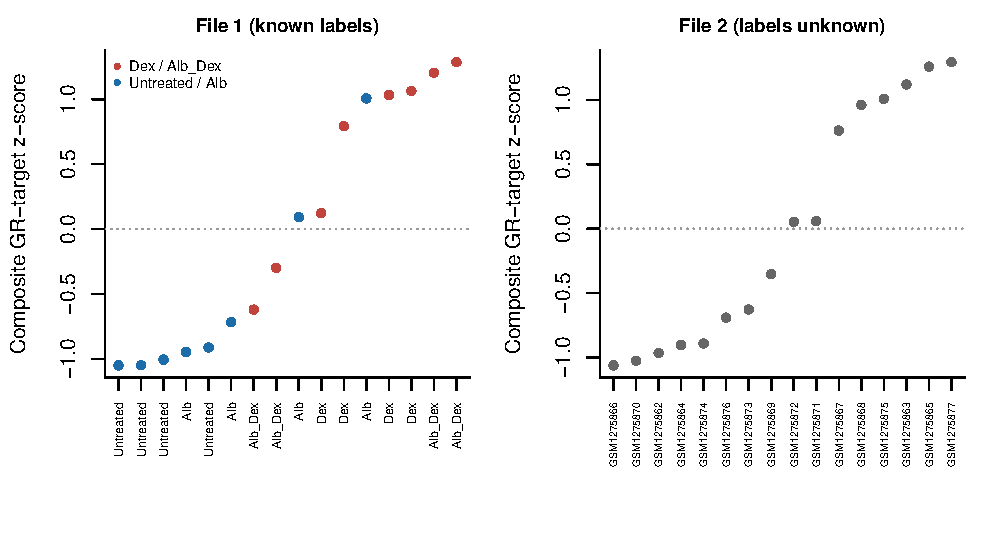
\includegraphics[width=\textwidth]{fig_marker_calibration.pdf}
\caption{Composite 8-marker GR-target $z$-score, one point per sample, sorted low to high. \emph{Left}: File 1, colored by true label -- Dex/Albuterol+Dex (red) versus Untreated/Albuterol (blue); note the label-color reversals in the middle of the sorted order, the source of the 75\% calibration accuracy. \emph{Right}: File 2, labels unknown, plotted in the same way for visual comparison; its middle-of-range ambiguity mirrors File 1's, which is why its two-cluster split is reported but not relied upon.}
\label{fig:calibration}
\figalttext[Two dot plots]{Sorted composite marker z-scores for 16 samples in each of two files, both showing a mostly-separated but partially ambiguous middle region.}
\end{figure*}

This is, in itself, a genuine and directly relevant finding: reproducing a published, heavily-cited dataset's differential-expression result from its re-processed public form is not just an identifier-mapping problem but can also be a metadata-preservation problem, and a literature-validated marker panel is not automatically sufficient to paper over missing metadata. We report it as what it is -- a calibration failure discovered honestly, rather than a positive result -- because a paper about auditing invisible failure modes in bioinformatics pipelines should not itself paper over one.

\section{Illustrative example}\label{sec:example}

\begin{boxtext}[Synthetic data notice]
Every number in this section is computed by the real \texttt{idmapaudit} functions described in Section~\ref{sec:fragility}, but the input significance calls themselves are hand-constructed toy data chosen to illustrate the three regimes the fragility score is designed to separate. They are \emph{not} derived from GSE52778, from any other real dataset, or from any real pathway database, and the pathway labels (\texttt{toy:*}) are placeholders, not real pathway identifiers. No biological claim should be attributed to this section.
\end{boxtext}

Fig.~\ref{fig:heatmap} shows a synthetic significance matrix for eight toy pathways across the six primary mapping branches of Section~\ref{sec:matrix}, and Table~\ref{tab:toy} shows the resulting fragility table, produced by \texttt{build\_fragility\_table()} on that matrix without modification. \texttt{toy:always\_on} and \texttt{toy:always\_off} are stable by construction ($H_p=0$); \texttt{toy:coin\_flip\_a/b} alternate every other branch, giving the maximal fragility $F_p=0.5$, $H_p=1$; the remaining four pathways each flip in exactly one of six branches ($F_p\in\{1/6,5/6\}$, $H_p\approx0.650$), illustrating a single-branch-driven fragility case -- exactly the pattern the versioned-Ensembl positive control (Section~\ref{sec:matrix}) is expected to produce at scale on real data. The mean pairwise Jaccard index of the significant-pathway sets across all $\binom{6}{2}=15$ branch pairs in this toy example is 0.591, reflecting that 6 of 8 toy pathways are not called consistently across every branch pair.

\begin{figure}[!t]
\centering
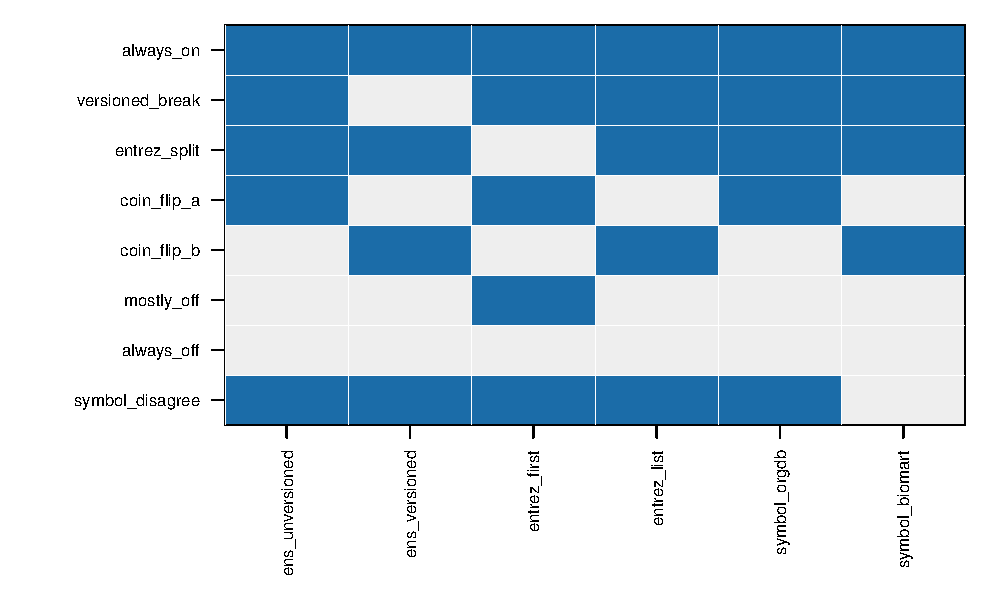
\includegraphics[width=\columnwidth]{fig_toy_heatmap.pdf}
\caption{Synthetic significance-call matrix (dark = significant) for eight illustrative toy pathways across six illustrative mapping branches. Hand-constructed to demonstrate the score's mechanics; not derived from real data (see boxed notice, Section~\ref{sec:example}).}
\label{fig:heatmap}
\figalttext[Binary heatmap]{An eight-row by six-column grid of dark and light cells representing synthetic significance calls, used only to illustrate the fragility-score calculation.}
\end{figure}

\begin{table}[!t]
\caption{Fragility table for the synthetic illustrative example (Fig.~\ref{fig:heatmap}), computed by \texttt{idmapaudit::build\_fragility\_table()}. $k_p$: testable branches; $F_p$: fragility proportion (Eq.~\ref{eq:fragility}); $H_p$: binary entropy (Eq.~\ref{eq:entropy}).\label{tab:toy}}
\begin{tabular*}{\columnwidth}{@{\extracolsep\fill}lcccl@{\extracolsep\fill}}
\toprule
Pathway (synthetic) & $k_p$ & $F_p$ & $H_p$ & Class \\
\midrule
toy:always\_on           & 6 & 1.000 & 0.000 & stable \\
toy:always\_off          & 6 & 0.000 & 0.000 & stable \\
toy:coin\_flip\_a        & 6 & 0.500 & 1.000 & fragile \\
toy:coin\_flip\_b        & 6 & 0.500 & 1.000 & fragile \\
toy:entrez\_split        & 6 & 0.833 & 0.650 & fragile \\
toy:mostly\_off          & 6 & 0.167 & 0.650 & fragile \\
toy:symbol\_disagree     & 6 & 0.833 & 0.650 & fragile \\
toy:versioned\_only\_break & 6 & 0.833 & 0.650 & fragile \\
\botrule
\end{tabular*}
\end{table}

\section{Discussion and limitations}\label{sec:limitations}

This manuscript reports what has actually been built and run: a fully specified and unit-validated stability-metric framework, a wired-up ID-mapping matrix and enrichment-battery interface, a real empirical case study on GSE52778's two independently-processed public forms (Section~\ref{sec:real}), and a synthetic illustration of the fragility-score mechanics (Section~\ref{sec:example}). It deliberately does not report pathway-\emph{level} findings (GO/KEGG/Reactome/WikiPathways fragility scores) on GSE52778 or any other dataset, because the Bioconductor packages the full empirical pipeline depends on (\texttt{DESeq2}, \texttt{org.Hs.eg.db}, \texttt{clusterProfiler}, \texttt{ReactomePA}, \texttt{biomaRt}, \texttt{fgsea}) remain network-unreachable in the environments used to prepare this manuscript -- CRAN and Bioconductor's package servers, and every live pathway/annotation data source checked (KEGG, Ensembl BioMart, Reactome, WikiPathways, g:Profiler, Enrichr, mygene.info), are all blocked by the sandbox's network egress policy, a restriction that granting in-conversation permission does not lift, since it is enforced outside the conversation. What could be recovered from source -- most core Bioconductor infrastructure and the \texttt{clusterProfiler} ecosystem are mirrored on GitHub, which the environment does permit -- was not sufficient, because the annotation \emph{data} packages (\texttt{org.Hs.eg.db}, \texttt{reactome.db}, \texttt{HDO.db}, and the Bioconductor \texttt{airway} data package itself) are not mirrored there, only Bioconductor \emph{software} packages are. The \texttt{targets} pipeline that would produce full pathway-level fragility scores is complete and reviewable in the linked repository, and is exercised as a continuous-integration smoke test in an environment where those packages can be installed; running it end to end against GSE52778 and the two additional planned datasets (GSE159094, a PBMC dexamethasone series, and GSE80651, a podocyte series) to answer whether pathway fragility is a property of the pathway's gene-set definition or of a single dataset's noise, and anchoring the glucocorticoid case study against ChIP-seq-derived GR/NR3C1 target gene sets, remains the immediate next step.

The real case study in Section~\ref{sec:real} was made possible only because the corresponding author supplied the two GSE52778 files directly; it illustrates, on genuine data, both halves of this project's concern -- a background-choice-sensitive gene-universe difference and real symbol-naming anomalies at the namespace/annotation level (Section~\ref{sec:real-universe}), and, in the calibration finding of Section~\ref{sec:real-calibration}, a related but distinct failure mode. We state that finding narrowly and deliberately: \emph{the supplementary FPKM matrix we analyzed does not carry per-sample treatment labels}, not that GSE52778's metadata is lost from the record. We were not able to check GEO's own series-level sample characteristics against this file (the sandbox this manuscript was prepared in has no network path to GEO/NCBI either), so we do not know whether the two would agree; if the series record does carry per-sample labels, as would be typical, the correct fix is to use them directly rather than infer treatment identity from expression, and the 75\% marker-panel accuracy we report is then a statement about a workaround's limits, not about the dataset's metadata. Either way, we did not build a headline fragility number on the recovered labels, because doing so would have reported label-recovery noise as if it were mapping-driven instability -- the same conflation Section~\ref{sec:design} designs against for the DE step, applied here to a workaround we would not have needed had the series metadata been available to us directly. For the same reason, Section~\ref{sec:real-de}'s differential expression uses an unpaired test despite GSE52778's paired donor design (each of four donors contributes all four treatments): the sample-to-donor correspondence is carried in the same series metadata we could not fetch, and guessing it would risk exactly the kind of confident-but-wrong labeling this paragraph just declined to build on. A paired re-analysis, and the real cross-namespace differential-expression comparison File 1 and File 2's shared samples would enable once correctly labeled, are immediate next steps that need only that metadata, not new code.

A second, related limitation is that the GSEA mode of the enrichment battery (Section~\ref{sec:design}) is interface-complete but not yet wired to a concrete pathway gene-set source (MSigDB Hallmark, C2:CP:KEGG, Reactome); only ORA is currently runnable end to end.

Finally, even once run on real data, three sources of instability must be kept analytically separate, as argued in Section~\ref{sec:fragility}: mapping-driven fragility, threshold-proximity flips that have nothing to do with identifier choice, and dataset-specific noise versus a pathway-intrinsic property. The framework reports the machinery to make each separation (threshold-sensitivity reporting, the mapping-noise null, and cross-dataset agreement), but none of that machinery substitutes for actually running it against real, independent datasets, which is future work.

\section{Conclusion}\label{sec:conclusion}

Gene-identifier-mapping choice is a routinely invisible step between differential expression and pathway enrichment. \texttt{idmapaudit} turns that choice into a measured, reusable quantity -- the per-pathway fragility score -- built on a stability-metric core that is fully specified, unit-tested against hand-computed answers, and released independently of the heavier Bioconductor dependencies its empirical use requires. Applied to real, public GSE52778 data, the same auditing mindset surfaced genuine findings beyond what was originally planned, including two corrections to our own first attempt at measuring them: a gene-universe difference between two public processings of the identical experiment that shrinks from 69\% to 3.7\% once an appropriately expression-filtered background is used instead of the naive raw-annotation count, a symbol-anomaly rate that shrinks from an overstated 11.3\% to a defensible 9.2\% once current, stable HGNC naming families are excluded, and a marker-based sample-relabeling method that only reaches 75\% accuracy even under calibration -- a workaround-fragility problem adjacent to, and compounding, the identifier-mapping problem this tool was built to audit. The tool is ready to run full pathway-level enrichment against real data as soon as it runs somewhere with Bioconductor annotation-data access; this manuscript reports its design and every result actually obtained honestly, including a negative calibration result, rather than results that were not obtained.

\section{Conflicts of interest}
The author declares no competing interests.

\section{Funding}
None declared.

\section{Data availability}
No new biological data were generated. All data analyzed are publicly available from the NCBI Gene Expression Omnibus under accession GSE52778 \citep{himes2014rnaseq}: the two files analyzed in Section~\ref{sec:real} (\texttt{GSE52778\_All\_Sample\_FPKM\_Matrix.txt} and \texttt{GSE52778\_norm\_counts\_FPKM\_GRCh38.p13\_NCBI.tsv}) are included in the linked repository under \texttt{analysis/gse52778-real/}, alongside the analysis script and its full output tables. The \texttt{airway} Bioconductor data package (a curated 8-sample subset of the same series) underlies the not-yet-executed \texttt{targets} pipeline of Section~\ref{sec:software}. All code, the methods note, the real-data analysis, and the synthetic illustrative-example data underlying Table~\ref{tab:toy} and Fig.~\ref{fig:heatmap} are available at \url{https://github.com/ethanyyy123/bioadvances}.

\section{Author contributions statement}
E.Y.Y.\ conceived the audit framework, directed its design and scope, supplied the GSE52778 data files analyzed in Section~\ref{sec:real}, reviewed and takes responsibility for the software, the analysis, and this manuscript's content and claims. Implementation of the software and tests, execution of the analyses, and drafting of the manuscript text were carried out by Claude (Anthropic), a generative-AI coding assistant, under E.Y.Y.'s direction and iterative review; see the Generative-AI use section below.

\section{Generative-AI use disclosure}
Claude (Anthropic; specifically Claude Sonnet 5, accessed via Claude Code) was used throughout this project's preparation: to write the \texttt{idmapaudit} R package and its test suite, to run the analyses in Sections~\ref{sec:real} and~\ref{sec:validation}, to draft this manuscript's text, and to revise the manuscript, code, and analysis in response to external review, including the specific corrections described in Section~\ref{sec:limitations}. The corresponding author directed the project's scope and design, supplied the real data analyzed, and reviewed the resulting code, analysis, and text, but did not independently re-derive every reported number by hand. Every commit in the linked repository is consequently attributed to "Claude" in its Git authorship metadata (visible in the repository's commit history) rather than to E.Y.Y.\ personally; we disclose this explicitly, following ICMJE and COPE guidance that generative-AI tools cannot be listed as authors and that their use in manuscript and code preparation must be stated rather than left for a reader to discover.

\bibliographystyle{oup-abbrvnat}
\bibliography{reference}

\end{document}
